\section{Dissusion}
\subsection{Unachieved implementation of chunks} \label{DiscussionChunks}
Memory efficiency and optimization has been a high priority since the start of Minion Map. We knew from the start of the project, that to be able to load Denmark would require efficient handling of heap space. Therefore it has always been a goal to filestream the inputted .OSM file into smaller \textit{chunks}. 
\subsubsection{What is the problem?}
The main objective with the chunks was to minimize the heap allocated from the KDTree, and only load in what part of the map the viewer sees. As mentioned in \ref{KDTree}, the current implementation of Minion Map uses the KDTree to draw all the content the viewer sees. But a big problem with this is that the KDTree always stores all parsed .OSM data in the heap at all times, even if the user only sees a small part of the .OSM data. This can lead to memory overflow when trying to load bigger .OSM files, such as Denmark. We knew this drawback from the start of the project, and therefore started the development of chunks at the same time as KDTrees. 
\begin{figure}[ht]%
  \centering
  \subfloat[\centering \textit{Representation of current KDTree implementation.}\label{chunks/impl1}]
  {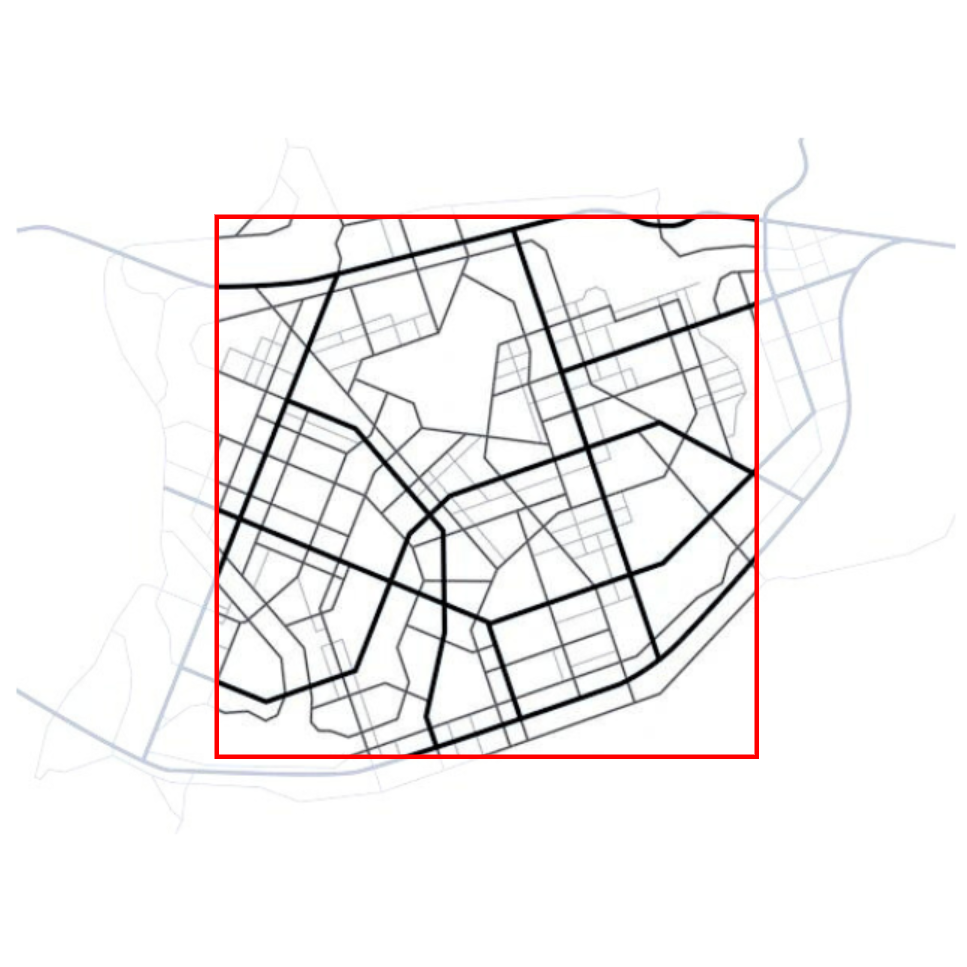
\includegraphics[width=8cm]{docs/material/chunksVizualication0.png}}
%
  \subfloat[\centering \textit{Representation of chunks}\label{chunks/impl2}]
  {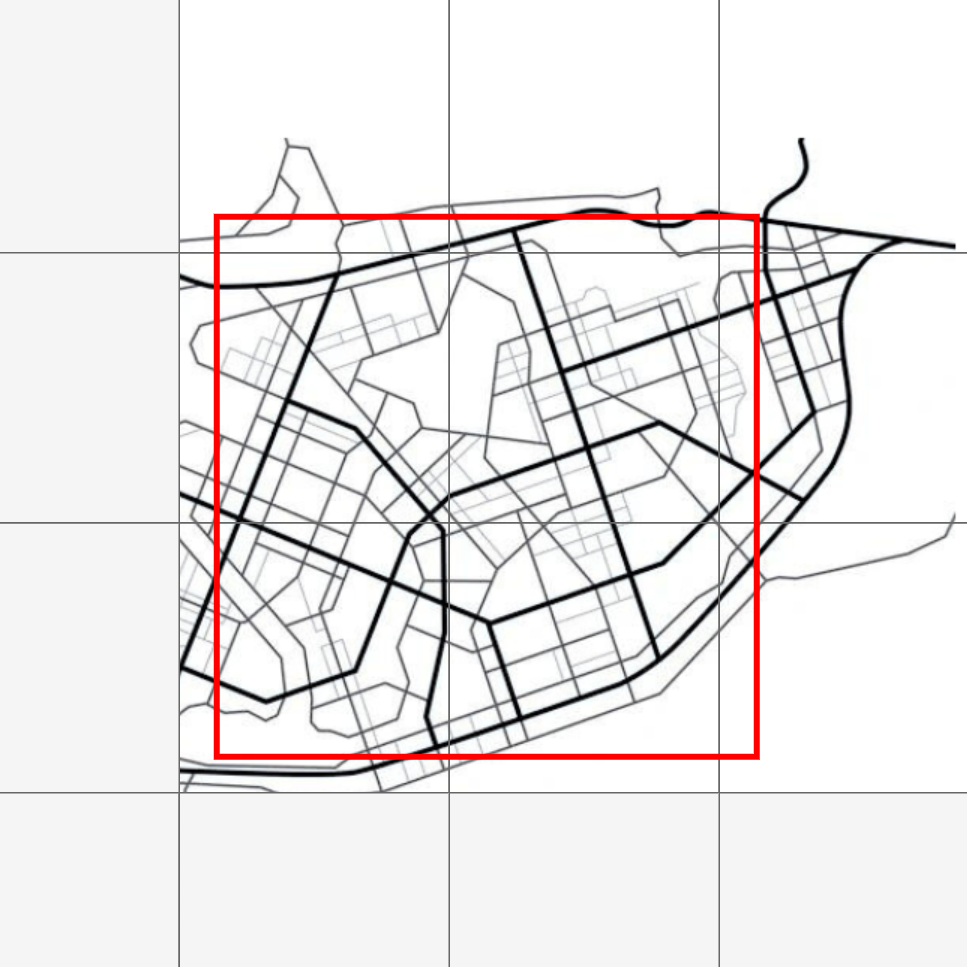
\includegraphics[width=8cm]{docs/material/chunksVizualication2.png}}%
  \caption{Illustrations of intended implementation of chunks}\label{chunks/implement}
\end{figure}
\newpage
The red box in figure \ref{chunks/implement} is the viewbox of what the user can see. Outside the viewbox in figure \ref{chunks/impl1} there are undrawn parts of the map that are still in the heap. The viewbox within the bounds of nine chunks in figure \ref{chunks/impl2} is, where all the map parts are loaded into the heap and drawn. The grey boxes are unloaded map chunks, that are loaded in at runtime, if the viewbox is within the bounds
\subsubsection{How did we implement it?}
When we implemented file streaming the data into chunks, we had multiple considerations for how the data should be stored into the chunks. To achieve as little memory allocation as possible, we chose to only store the TagBound of the chunks area and all the Tag-Nodes and Address’ that were within the bound. 
\newline
But this solution leads to a problem when we want to draw ways and relations. How do we draw a way if only we have loaded a single TagNode in from the chunk?

\begin{figure}[ht]%
  \centering
  \subfloat[\centering Illustration of problem to draw a TagWay from an isolated TagNode in a chunk.\label{chunks/problem}]{{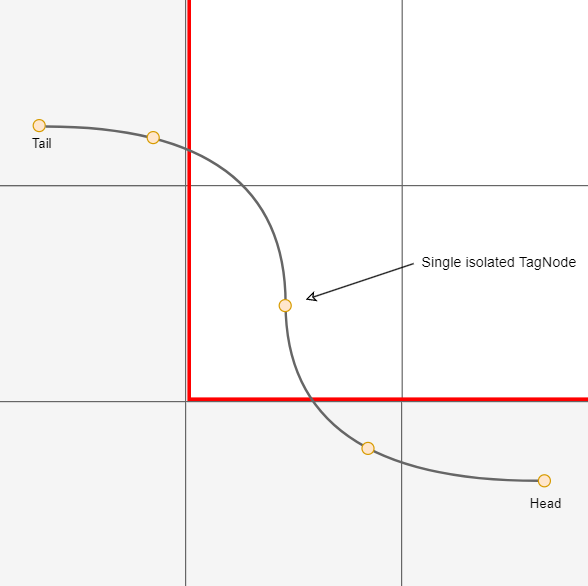
\includegraphics[width=6.5cm]{docs/material/ChunksProblem.png}}}
  \hspace{2cm}
  \subfloat[\centering Illustration of the solution with the use of Double-Linked-List. \label{dis/withChunks}]{{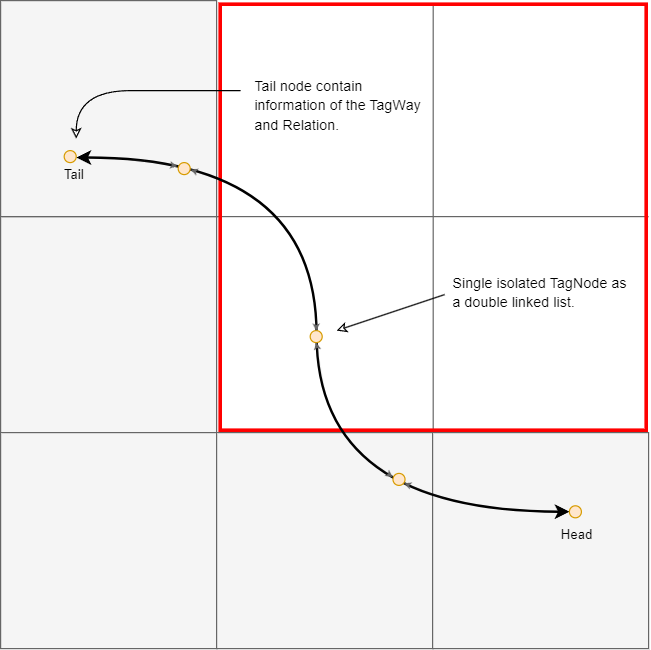
\includegraphics[width=6.5cm]{docs/material/ChunkSolution.drawio.png}}}
  \caption{Illustration of problem cause and solution for chunks }\label{kbhBench}
\end{figure}
The path in figure \ref{chunks/problem} is not drawable because the isolated TagNode has no reference to the other nodes in the TagWay, so how did we solve this?
\\
As mentioned in section \ref{section/parser} about the parser, we have made the TagNodes compatible to be in a double linked list, to solve this exact problem. This would allow a single isolated TagNode to draw its corresponding TagWay, just by going back to its previous node until the tail node has been reached. Because the TagWay object is connected to the tail node of a way, can the full list of tags in the way be read with all the attributes of the TagWay.  TagRelations are at the same time connected to TagWay’s the same way as TagWays are connected to TagNodes. That is how all the information of the corresponding TagWay and TagRelation can be read from one single isolated TagNode in the chunk.
\par
Another problem to face is being able to load the right chunks quickly. Instead of iterating through all of the 256 chunks that were made from the original .OSM file, we chose to use the KDTree to chunk what chunks were inside the viewport. This would allow us to read what chunks needed to be loaded in $O(\log n)$ time.
\subsubsection{What went wrong and was it beneficial?}
When the code was ready to be run a week before the due date, we found a lot of trouble with the new implementation. The ability to filestream and write the objects to binary worked great, but not when it came to reading the data again. We quickly found out that the amount of references in the TagNodes came at a cost. When reading the TagNodes from the chunks, the stack overflew with references. We therefore could not load any larger .OSM files, without manually increasing the maximum stack size that the program was allowed to use. Only then were we able to load large .OSM files, and benchmarks looked promising.

\begin{figure}[ht]%
  \centering
  \subfloat[\centering Benchmark of Copenhagen without chunks, tested one week before the due date.\label{dis/withoutChunks}]{{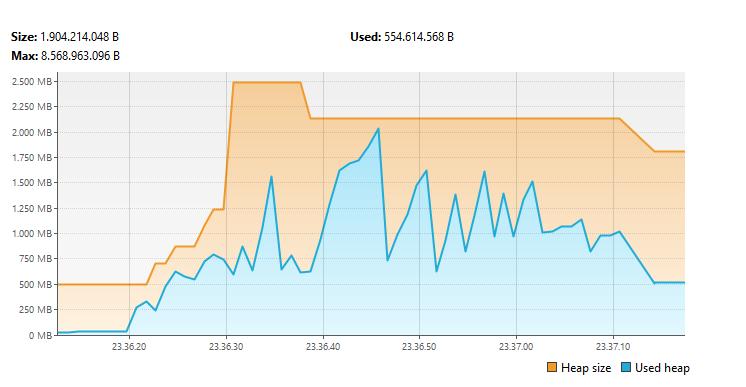
\includegraphics[width=8.25cm]{docs/material/KBHChunkingWithOutChunks.png}}}
  \subfloat[\centering Benchmark of Copenhagen with chunk, tested one week before the due date. \label{dis/withChunks}]{{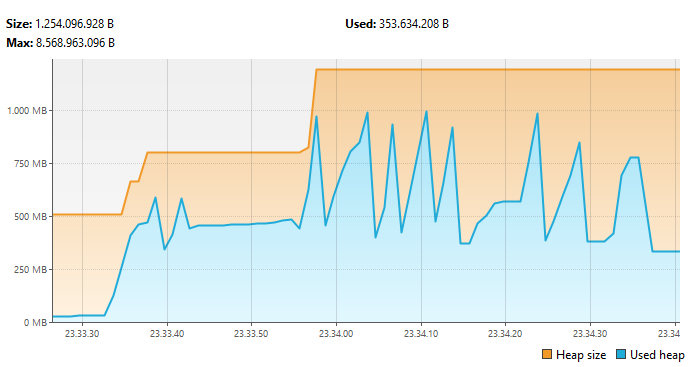
\includegraphics[width=8.25cm]{docs/material/KBHChunkingWithChunks.png}}}
  \caption{VisualVM benchmark tests of Copenhagen, with or without chunks}\label{kbhBench}
\end{figure}
\begin{table}[ht]
  \centering
  \begin{tabular}{ c|c|c|c }
   \textbf{Heap-dump of Benchmark} & \textbf{Heap Size} & \textbf{Classes} & \textbf{Instances}\\
   \hline
   Benchmark \ref{dis/withoutChunks} & $522.994.496$ B & $6.030$ & $12.233.209$ \\
   Benchmark \ref{dis/withChunks} & $320.652.472$ B & $6.079$ & $5.564.363$ \\
  \end{tabular}\\
  \caption{\centering Heap-dump for the two benchmarks in figure \ref{kbhBench}}\label{KDTree/timeComplexity}
\end{table}
The benchmarks show the chunked version of the application to be significantly more memory efficient than with the version that uses the KDTree. The chunked version's average memory usage is around 450-500 MB, with spikes that do not go above 1 GB when new chunks are loaded in. The chunked version used >75\% less average memory and had a reduction of 60\%-66\% less memory from the peaks of the two benchmarks. The real reason for this large memory reduction can be seen when comparing the two heap dumps- The difference between the amount of instances in the two benchmarks was also reduced by 87\%. 
\subsubsection{What are we left with?}
The implementation with chunks seemed promising from a memory perspective, but was not from a practical standpoint. The stack overflow problem was the largest one, and if that needed to be solved efficiently, we would need to refactor a large amount of the application. If we refactored the double-linked TagNodes into primitive arrays or another type, we would need to refactor many other components in the application. This would mean that we also need to refactor how the KDTree handles ways, how relations are drawn, the chunk builder and other components. This would at the same time set us back to having the same problem that made us switch to double-linked-list in the first place, and there was just no time for that. 
We therefore changed our focus away from the chunking implementation and focused on optimizing the KDTree to handle and draw data from the .OSM file. 
\subsection{Trie and searching}
Throughout different iterations of development, different ways of searching were used. Initially it was almost entirely based on regex. A regex which split a string into different matcher groups was used to determine what part of the searched string would correspond to the street, house number, city and so on. \\
Levenshtein distance is a way to measure how close one string is to another. An algorithm to find the Levenshtein distance and comparing two strings was implemented to help this, as it improved the searching, when the user didn’t write the address exactly as it was saved in the program. To utilize this, every address street and city were saved in ArrayLists, which were all compared to the searched string, until a suitable suggestion could be made. \\
After implementing the Trie, much of the former search class functionality was removed, as it was not compatible with the current vision. A lot of the functionality of the search class was moved to the Trie. Most of the address searching functionality was split up between the controller, the Search class and the SearchAddress class. It ended up being a lot more condensed, with the Search class doing significantly less, while the SearchAddress was removed entirely. \\
In hindsight, there could probably have been a way to preserve the Levenshtein distance algorithm, as it still might have improved the user experience when searching, as t would have enabled the user to still see results regardless of a misspelling. However it would also make searching slower, as more computations would be needed for every search. As the search method is called every time a character is added and then the Trie search, it could potentially cause performance issues when the user is typing. The method comparing Levenshtein distances takes two strings as arguments, which means that all addresses would have to be compared with the specified string. This could again be compared with specific streets saved in ArrayLists as was previously tried.
\subsection{Memory optimization}
One problem with objects created in the Java language, is the object overhead. When objects are created in Java, it contains something called object overhead, which is a term used for the data created along with the objects. The data included in the object overhead is for our case mostly unused. Therefore it would be best for us to utilize primitive data types frequently as possible. This means that when using the built in java.util.HashMap we are forced to use objects as both key and value. Whereas with the library GNU.Trove.map.TLongObjectHashMap library, the keys are stored as primitive data types in one array, which eliminates the object overhead for the keys.
\newline
Generally most of Java’s standard library uses objects in their data structures instead of primitive types, which through the eyes of memory optimization is not ideal. Therefore when it is possible to use a data structure that utilizes primitive data types instead of objects, we are obligated to do so. This implies when using HashMaps, ArrayLists and LinkedLists.
\newline
If we want to calculate the saved byte size when using primitive data types instead of objects, which is important when measuring the memory saved. We will have to tally the byte size per instance. For the primitive data type long, it is a 64-bit signed integer, which means the amount of byte it takes up in memory is 8, whereas the calculation for a Long object is different. Every object has a header which is 12 bytes and the accompanying data, which in this case is the primitive data type long that takes 8 bytes. Besides the object, we also need a reference to the object as it gets stored in a different place in the heap, this reference takes up 4 bytes of memory. Therefore the sum of a Long object is 24 bytes.\cite{memory/objects}
\begin{table}[ht]
  \centering
  \begin{tabular}{ c|c|c }
   \textbf{Type} & \textbf{Bytes in total} & \textbf{Comparison}\\
   \hline
   Primitive Long & $8$ & $\sim33\%$ \\
   Object Long & $24$ & $300\%$ \\
  \end{tabular}\\
  \caption{\centering A table of the comparison between object Long and primitive long}
\end{table}
As seen in the table above there is a $\sim$66\% saving of memory when using the primitive data type long instead of object Long.
\newline
Other than selecting the correct data structure to store data, it is important to only store data once and not referring to an object multiple times. When we read the data from the .OSM file, the data is stored in the XMLReader class, which is then transferred to the KDTree and deleted from the XMLReader. Which eliminates the duplicate references inside of our program.
\newline
\textbf{Model}
The primary thing found in the heap is our parsed data and our data structures filled up with that data. Thus, it had to be secured that there were no unused duplications of that data in the memory. This is why the class is a singleton object which is only able to have one single instance and is currently the only class where an instance of the XMLReader is constructed. The data within the tree consists of our relations and ways. These two collections are the ones that fill the most within our heap, therefore we clear them from the XMLReader after parsing them into the static Tree class fields. All remaining static fields are brought up to the singleton instance of Model and then cleared in the XMLReader, ensuring no possibility of having unused duplicates in the heap.\par
This initialization of the tree itself is very time consuming and fragile due to the amount of data. Therefore we use multi-threading inside of the Model class to load the KDTree. Each thread has its own stacksize and multiple threads can run at the same time, which has allowed us to load multiple datasets into the tree at the same time, cutting costs on load time for the tree.
\newline
\textbf{Pre-loaded model in Binary-file}
One of the formal requirements was to include a default binary file, which was somewhat achieved, just not the way we wanted it to be done. The model class has been created because of the many benefits there could have been by serializing the class into a file. As previously stated the model class ties up everything that has happens outside the view of the user. By having connected to all components, we could have serialized and outputted all of the needed processed data into a binary file, having substantially better load time on the included default files. But it did not make it to the final product due to serialization of our relations causing stack overflows. We suspect it might be caused by the use of LinkedLists. But due to the lack of time, we chose to focus on other parts of the program.




